
%\renewcommand{\Titulo}{A prototype of Automatic Book Digitalization System~}


\begin{frame}{\citetitle{MarcoNuno_CongArbIng_2014_12_00X}  (1)}
%\note[item]{\scriptsize The next project in my presentation is called \textit{A prototype of Automatic Book Digitalization System}}
%\note[item]{\scriptsize Book scanning is the process of taking a physical book and converting into a digital document (such as PDF or other formats). }
%\note[item]{\scriptsize One alternative is using flatbed scanners to acquire images of the book. These scanners require human intervention, and scanning each page are slow when a high defition image of each page is required}
%\note[item]{\scriptsize There are several alternatives, but most of them require expensive hardware components}
%\note[item]{\scriptsize In this project, we proposed a book scaning machine with the following hardware components}
%\note[item]{\scriptsize 1) Illumination System - based on LED light}
%\note[item]{\scriptsize 2) Book scanning support, made from a sheet of acrylic and painted in black.}
%\note[item]{\scriptsize 3) Camera, which performs the image acquisition using a PTP (Picture Transfer Protocol) to transfer the captured image to the processing platform. We used a Canon EOS rebel T3i camera}
%\note[item]{\scriptsize 4) Mechanical page turner system, which automatically turns the page after each image acquisition} 
%\note[item]{\scriptsize 5) Processing platform, where a Raspberry-Pi processing. This platform controls when the camera captures a photo of the book, and when the mecharican page turner must advance to digitalize the next page. The processing platform hosts the image processing system to perform the required processing to generate the digital version of the scanned book.}
%\note[item]{\scriptsize We published the presented results in the conference paper shown at the bottom of this slide.}

\note[item]{\scriptsize Book scanning is the digitalization of a printed book to obtain a digital version of this document. }
\note[item]{\scriptsize One alternative is using flatbed scanners to acquire images of the book. These scanners require human intervention, and scanning each page is slow since a high definition image of each page is required }
%\note[item]{\scriptsize }
\note[item]{\scriptsize In this project, we proposed a book scanning machine with the following low-cost hardware components: }
\note[item]{\scriptsize I) Illumination System - based on LED lights.}
\note[item]{\scriptsize II) Book scanning support, made from a sheet of acrylic and painted in black.}
\note[item]{\scriptsize II) Camera, which performs the image acquisition and transfer the captured image to the processing platform. We used a Canon EOS rebel T3i camera }
\note[item]{\scriptsize IV) Mechanical page-turner system, which automatically turns the page after each image acquisition }
\note[item]{\scriptsize V) Processing platform (a Raspberry Pi device). This platform controls when the camera captures a photo of the book pages and when the mechanical page-turner must advance to acquire the next page. The processing platform hosts the image processing system to perform the required processing to generate the digital version of the scanned book.}
%\note[item]{\scriptsize 10. We published the presented results in the conference paper shown at the bottom of this slide.}





\begin{block}{Hardware Materials} 


\begin{columns}
\begin{column}{0.35\textwidth}
		\begin{itemize}
		\item Illumination System
		\item Book Scanning Support
		\item Camera (Canon EOS rebel T3i)
		\item Mechanical page turner system
		\item Processing platform (Raspberry Pi)		
		\end{itemize}
		\begin{center}
		
        \end{center}
\end{column}
\begin{column}{0.43\textwidth}  
     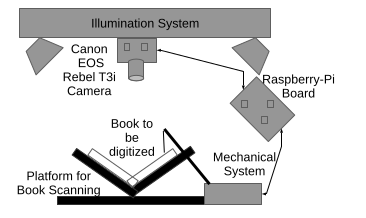
\includegraphics[width=0.95\textwidth]{Figs/BookScanner1}
\end{column}
\begin{column}{0.23\textwidth}  
    %\begin{center}
     %%%%% this is a minipage, so \textwidth is already adjusted to the size of the column

          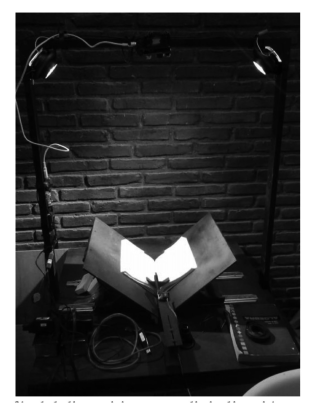
\includegraphics[width=0.95\textwidth]{Figs/BookScanner2}
     %\end{center}
\end{column}
\end{columns}
\end{block} 
%\footnotetext{Victor Rodríguez-Osoria, Marco Aurelio Nuño-Maganda, Yahir Hernández-Mier, and Cesar Torres-Huitzil. \textbf{Embedded Image Processing System for Automatic Page Segmentation of Open Book Images}. In Advances in  Visual Computing,  volume 8888  of Lecture Notes in Computer Science, pages 531-540. Springer International  Publishing, Diciembre 2014.  \url{http://dx.doi.org/10.1007/978-3-319-14364-4_51} }
%\setcounter{footnote}{0}
\footnotetext[1]{\fullcite{MarcoNuno_CongArbIng_2014_12_00X}}
\setcounter{footnote}{0}
\end{frame}


\begin{frame}{\citetitle{MarcoNuno_CongArbIng_2014_12_00X}  (2)}

% Slide 2
\note[item]{\scriptsize Operation required to segment both left and right pages: }
%\note[item]{\scriptsize 1) The input image is downsampled to speedup the image processing operators. }
%\note[item]{\scriptsize 2. A color conversion from RGB to Grayscale color space is performed in order to reduce image depth.}
%\note[item]{\scriptsize 3. A blurring median filtering is applied to remove noise and some details, and to help in the edge detection process.}
%\note[item]{\scriptsize 4. A morphological dilation is applied to fill holes and to obtain coarser edges.}
%\note[item]{\scriptsize 5.- Hough line detection is computed to find relevant information about lines in the image}
%\note[item]{\scriptsize 6.- A geometrical analysis of the obtained image is performed to find the four corners of each page. When the candidate corners are obtained, a second analysis is performed in order to validate the corners position.}
%\note[item]{\scriptsize 7.- An interpolation process for obtaining the image coordinates of each corner in the original image is computed.}
%\note[item]{\scriptsize 8. A perspective transformation is applied to the original image using the obtained corners from the previous step to correct the geometrical distortion of scanned pages.}



\begin{block}{Computation steps of the proposed system} 
\begin{columns}
\begin{column}{0.5\textwidth}
		\begin{itemize}
		\item The camera captures the book image and transfers to the procesing platform (PP). 
		\item The PP performs image processing operators to isolate left and right page.
		\item Once that each page (left and right) have been obtained, this pages are added to a PDF document
		\item The procesing platform activates the page turner to go to the next page.
		\end{itemize}
\end{column}
\begin{column}{0.5\textwidth}  
    \begin{center}
     %%%%% this is a minipage, so \textwidth is already adjusted to the size of the column
     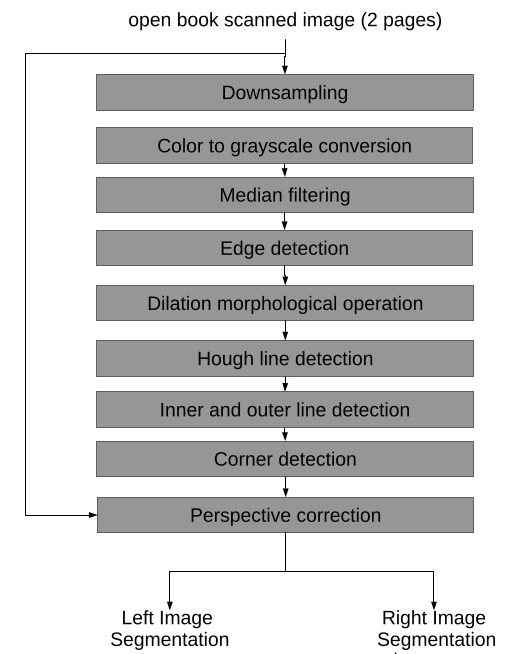
\includegraphics[width=0.60\textwidth]{Figs/DiagramaABloques_Escaner}

     \end{center}
\end{column}
\end{columns}
\end{block} 
\end{frame}


\begin{frame}{\citetitle{MarcoNuno_CongArbIng_2014_12_00X}  (3)}

% Slide 3
\note[item]{On the left we shown results related to the image processing performed to a input image. Original images is shown in (a), the bluring the image is shown in (b), the edge image is shown in (c), and in (d), the estimation of eight key corners that will be used for the page extraction is shown.}
\note[item]{On the right, we show a table with several digitalized pages and the resulting pages extracted  of each page using the image procesing operators previusly described.}
\note[item]{With the current system, it is possible to ditalize a maximum of eight 8 pages per minute (obtained from 4 book images). For a 800 pages book, we estimated a digitalization time of 100 minutes (1:40) without human intervention .}
\begin{block}{Results}  
\begin{columns}
\begin{column}{0.5\textwidth}
%   some text here some text here some text here some text here some text here
     \begin{center}
     %%%%% this is a minipage, so \textwidth is already adjusted to the size of the column
     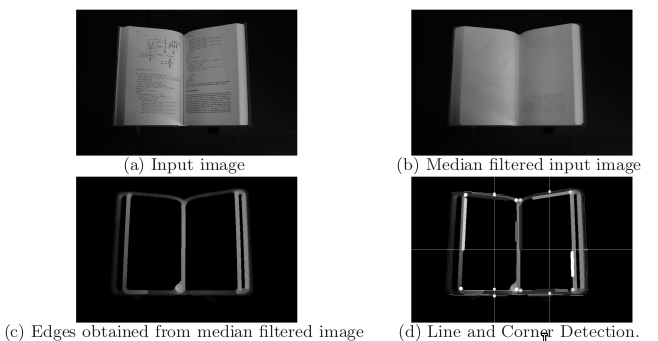
\includegraphics[width=0.98\textwidth]{Figs/BookScanner3}
     \end{center}

\end{column}
\begin{column}{0.5\textwidth}  
    \begin{center}
     %%%%% this is a minipage, so \textwidth is already adjusted to the size of the column
     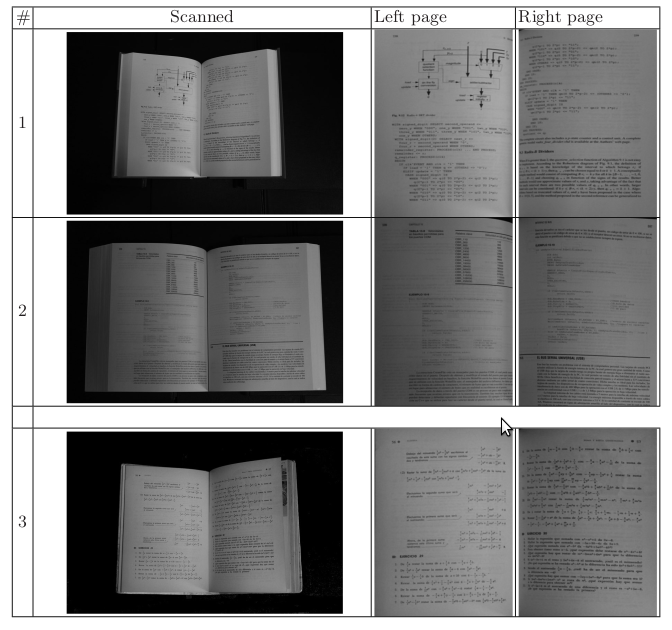
\includegraphics[width=0.88\textwidth]{Figs/BookScanner4}
     \end{center}
\end{column}
\end{columns}
\end{block} 
\end{frame}

